\section{Dirichlet边值问题}
\sourcepage{175--176}
此前的全纯、亚纯函数存在定理本质上依赖Dolbeault引理和有限性定理。现在用完全独立的Perron方法解决调和函数的Dirichlet问题。
\entry{22.1}{}
可微函数$u$调和是指$d'd''u=0$，在坐标$z=x+iy$中等价于$u_{xx}+u_{yy}=0$。单连通区域上的实调和函数是全纯函数的实部：由(19.4)，调和形式$du$为某全纯形式的实部，再积分得$du=\operatorname{Re}(dg)$，故$u=\operatorname{Re}g+\text{常数}$。

由此得调和函数最大值原理：区域上的实调和函数若在内部取到最大值，必为常数。局部写$u=\operatorname{Re}f$，则$|e^f|=e^u$在同点取最大值，由全纯函数最大值原理知局部为常数，再由连通性在全域为常数。
\entry{22.2}{}
\textbf{Dirichlet问题}：给定开集$Y\subset X$及连续$f:\partial Y\to\R$，求$\overline Y$上的连续函数$u$，在$Y$内调和且边界值为$f$。若$\overline Y$紧且边界非空，解若存在就唯一，因为两解之差边界为零，最大值原理给出其既$\le0$又$\ge0$。

对圆盘$D(R)$，可用Poisson积分求解。
\entry{22.3}{定理}
对连续边界函数$f$，令
\begin{equation}u(z):=\frac1{2\pi}\int_0^{2\pi}\frac{R^2-|z|^2}{|Re^{i\theta}-z|^2}f(Re^{i\theta})d\theta\quad(|z|<R),\tag{*}\end{equation}
边界上令$u=f$。则$u$在闭圆盘上连续，在内部调和。
\begin{proof}
对$z\ne\zeta$令$P(z,\zeta):=(|\zeta|^2-|z|^2)/|\zeta-z|^2$、$F(z,\zeta):=(\zeta+z)/(\zeta-z)$，则$P=\operatorname{Re}F$。
\sourcepage{177}
故$u$为全纯函数
\[\frac1{2\pi i}\int_{|\zeta|=R}F(z,\zeta)f(\zeta)\frac{d\zeta}{\zeta}\]
的实部，因而调和。留数定理给
\[\frac1{2\pi}\int_0^{2\pi}P(z,Re^{i\theta})d\theta=1.\]
固定$\zeta_0$在边界，则
\[
u(z)-f(\zeta_0)=\frac1{2\pi}\int_0^{2\pi}P(z,\zeta)(f(\zeta)-f(\zeta_0))d\theta.
\]
给定$\varepsilon$，取$\delta_0$使$|\zeta-\zeta_0|\le\delta_0$时函数值差$\le\varepsilon/2$。设$|f|\le M$，把圆周分为近、远两部分。近部分积分绝对值$\le\varepsilon/2$；若$\delta:=|z-\zeta_0|\le\delta_0/2$，远部分有$|\zeta-z|\ge\delta_0/2$，且$R^2-|z|^2\le2R\delta$，所以
\[
|u(z)-f(\zeta_0)|\le\varepsilon/2+16RM\delta/\delta_0^2\le\varepsilon
\]
当$\delta$足够小。故边界连续。
\end{proof}
\sourcepage{178}
\entry{22.4}{推论}
圆盘上的调和函数满足：对$r<R$、$|z|<r$，$u(z)=\frac1{2\pi}\int_0^{2\pi}P(z,re^{i\theta})u(re^{i\theta})d\theta$。特别地有均值性质$u(0)=\frac1{2\pi}\int_0^{2\pi}u(re^{i\theta})d\theta$。由解的唯一性及(22.3)得到。
\entry{22.5}{推论}
调和函数列在紧子集上一致收敛的极限仍调和。
\begin{proof}
在半径$r<R$的圆周上一致收敛，可在(22.4)中取极限，故极限仍满足Poisson公式，由(22.3)调和。
\end{proof}
\entry{22.6}{Harnack定理}
若$u_0\le u_1\le\cdots\le M$为圆盘上的调和函数列，则在每个紧子集上一致收敛于调和函数。
\begin{proof}
对紧集选$K\subset\{|z|\le\rho\}$，$\rho<r<R$。令$\varepsilon'=\varepsilon(r-\rho)/(r+\rho)$。由$u_n(0)$单调有界，$n\ge m\ge N$时$u_n(0)-u_m(0)\le\varepsilon'$。对正调和函数差应用Poisson公式，并用$0\le P(z,re^{i\theta})\le(r+\rho)/(r-\rho)$，
\sourcepage{179}
得$0\le u_n(z)-u_m(z)\le\frac{r+\rho}{r-\rho}(u_n(0)-u_m(0))\le\varepsilon$。故一致收敛，再用(22.5)。
\end{proof}
\entry{22.7}{}
调和性在双全纯映射下不变，因此位于坐标卡内、坐标像为圆盘的相对紧区域均可解Dirichlet问题。对开集$Y$，以$\operatorname{Reg}(Y)$表示对任意连续边界数据均可解此问题的相对紧子区域$D$。对连续实函数$u$，令$P_Du$在$Y\setminus D$等于$u$，在$D$内为相应调和解。显然此算子线性、保持不等式；$u$调和当且仅当对所有$D$有$P_Du=u$。
\entry{22.8}{定义}
连续实函数$u$称为\textbf{次调和}，若所有$D\in\operatorname{Reg}(Y)$均满足$P_Du\ge u$。次调和函数的和、非负常数倍及两函数的最大值仍次调和。若每点附近次调和，称为局部次调和。
\entry{22.9}{定理（局部次调和函数最大值原理）}
区域上局部次调和函数若在内部取最大值，则为常数。
\sourcepage{180}
\begin{proof}
令最大值为$c$，$S:=\{u=c\}$。若$S\ne Y$，选$a\in\partial S\cap Y$。连续性给$u(a)=c$，每个邻域中有值$<c$的点。可选$a$的正则圆盘邻域$D$，使边界值不恒为$c$，且$u$在$\overline D$附近次调和。则$u\le v:=P_Du$，而边界$v\le c$，故内部$v\le c$。由$v(a)\ge c$，$v$在内部取最大值，必恒为$c$，与边界选择矛盾。
\end{proof}
\entry{22.10}{推论}
局部次调和等价于次调和。
\begin{proof}
对任意$D$，$v=u-P_Du$在$D$局部次调和，边界为零，由最大值原理$v\le0$。
\end{proof}
\entry{22.11}{引理}
若$u$次调和且$B\in\operatorname{Reg}(Y)$，则$P_Bu$仍次调和。
\begin{proof}
令$v=P_Bu$。对任意$D$，在$Y\setminus D$有$P_Dv=v$；在$Y\setminus B$有$P_Dv\ge P_Du\ge u=v$。故$v-P_Dv\le0$于$Y\setminus(B\cap D)$，而它在$B\cap D$调和，由最大值原理内部也$\le0$。
\end{proof}
\entry{22.12}{Perron引理}
设$M$为非空连续次调和函数族，满足(i)对两函数取最大值封闭；(ii)对所有$P_D$封闭；(iii)存在常数$K$为共同上界。则$u^*(x):=\sup_{u\in M}u(x)$调和。
\sourcepage{181}
\begin{proof}
固定$a$及其正则圆盘邻域$D$。取$u_n\in M$使$u_n(a)\to u^*(a)$；通过有限最大值可假设单调递增。令$v_n=P_Du_n$，由Harnack定理在$D$趋于调和$v$，且$v(a)=u^*(a)$、$v\le u^*$。

任取$x\in D$，再取$w_n\in M$使$w_n(x)\to u^*(x)$。用最大值及$P_D$替换，可假设$w_n\le w_{n+1}$、$w_n\ge v_n$且在$D$调和。其极限$w$调和，$v\le w\le u^*$。在$a$相等，由最大值原理$w=v$，所以$v(x)=u^*(x)$。$x$任意，故$u^*$在$D$调和。
\end{proof}
\entry{22.13}{}
给定有界连续$f:\partial Y\to\R$，不要求$\overline Y$紧，令$K:=\sup_{\partial Y}f$。
\sourcepage{182}
\textbf{Perron族}$\mathcal P_f$由所有$\overline Y$上的连续函数组成，要求在$Y$次调和，边界$u\le f$，整体$u\le K$。由引理，其上确界$u^*$在$Y$调和。要成为边值问题的解，还需每个$x\in\partial Y$处$\lim_{y\to x,y\in Y}u^*(y)=f(x)$；这一般不总成立。
\entry{22.14}{定义}
若边界点$x$有开邻域$U$及$\overline Y\cap U$上的连续函数$\beta$，在$Y\cap U$次调和，且$\beta(x)=0$、其他点$\beta<0$，称$x$\textbf{正则}，$\beta$称为该点的\textbf{障碍函数}。若$Y_1\subset Y$开且$x\in\partial Y_1$，则同一障碍仍适用。因此正则边界的每个连通分支也有正则边界。
\entry{22.15}{引理}
若$x$为正则边界点，$V$为其邻域，$m\le c$为实常数，则存在$\overline Y$上连续、$Y$内次调和的$v$，使$v(x)=c$、$v|_{\overline Y\cap V}\le c$、$v|_{\overline Y\setminus V}=m$。
\begin{proof}
可设$c=0$。取障碍$\beta$及其定义邻域$U$，缩小$V$使$V\Subset U$，则$\sup_{\partial V\cap\overline Y}\beta<0$。选$k>0$使该边界上$k\beta<m$。
\sourcepage{183}
在$\overline Y\cap V$令$v=\max(m,k\beta)$，外部令$v=m$。它连续且局部次调和，因而次调和，满足各条件。
\end{proof}
\entry{22.16}{引理}
Perron上确界在每个正则边界点趋于指定边界值。
\begin{proof}
给定$\varepsilon>0$，取$x$的相对紧邻域$V$使$|f(y)-f(x)|\le\varepsilon$于$\partial Y\cap V$。设$k\le f\le K$。
(a)由(22.15)，取$v$在$x$值为$f(x)-\varepsilon$，在$V$上不超过此值，外部等于$k-\varepsilon$。则$v\in\mathcal P_f$，所以$\liminf u^*\ge f(x)-\varepsilon$。
(b)取次调和$w$，$w(x)=-f(x)$，在$V$上$w\le-f(x)$，外部等于$-K$。对每个$u\in\mathcal P_f$，在$\partial Y\cap V$有$u+w\le\varepsilon$，在$\overline Y\cap\partial V$有$u+w\le0$。
\sourcepage{184}
由最大值原理，在$Y\cap V$有$u+w\le\varepsilon$，故$\limsup u^*\le\varepsilon-w(x)=f(x)+\varepsilon$。合并并令$\varepsilon\to0$。
\end{proof}
\entry{22.17}{定理}
若$Y$的全部边界点正则，则对每个连续有界边界函数，Dirichlet问题可解。由(22.16)直接得到。

下面给出保证正则性的简单几何条件。正则性局部且双全纯不变，只需对平面陈述。
\entry{22.18}{定理}
若$a\in\partial Y$，存在圆盘$D=\{|z-m|<r\}$使$a\in\partial D$且$\overline D\cap Y=\varnothing$，则$a$为正则边界点。
\begin{proof}
令$c=(a+m)/2$，则$\beta(z):=\log(r/2)-\log|z-c|$为$a$处障碍，见图6。
\end{proof}
\begin{center}\begin{minipage}{\linewidth}\centering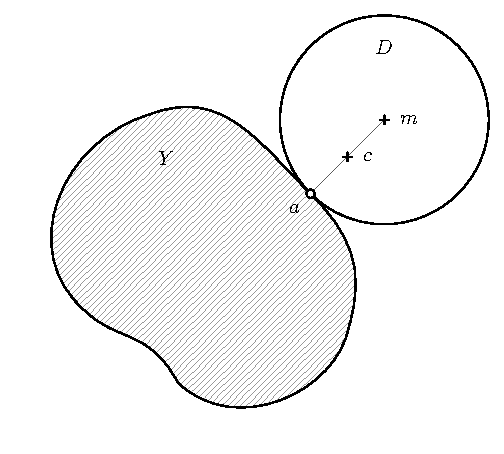
\includegraphics[width=.42\textwidth]{figures/fig06-tikz.pdf}\\图6\end{minipage}\end{center}
\sourcepage{185}
\subsection*{习题（第22节）}
\entry{22.1}{}
设$u\ge0$在$D(R)$调和。证明Harnack不等式$\frac{R-|z|}{R+|z|}u(0)\le u(z)\le\frac{R+|z|}{R-|z|}u(0)$。
\entry{22.2}{}
用Harnack不等式证明：整个复平面上有上界的实调和函数为常数。
\entry{22.3}{}
若连续实函数在$Y\subset\C$的每个闭圆盘上满足$u(a)\le\frac1{2\pi}\int_0^{2\pi}u(a+re^{i\theta})d\theta$，证明它次调和。
\entry{22.4}{}
若$a\in\partial Y$且存在从$a$出发的非退化线段$S$满足$S\cap Y=\varnothing$，证明$a$为正则边界点。
